%\documentclass[compress]{beamer}
\documentclass[compress,handout]{beamer}

%%%%% PREAMBLE %%%%%

% we want to draw diagrams (turns out not like this though)
\usepackage{tikz}

% figures in a presentation look better without "Figure"
\usepackage{caption}
\captionsetup[figure]{labelformat=empty}

%% % for Idris syntax highlighting
%% \usepackage[styles]{idrislang}

\usepackage{minted}
\setminted{
  fontsize=\small,
  breaklines=true
}

% slide url at the end
\usepackage{hyperref}
\hypersetup{
  colorlinks=true,
  urlcolor=purple
}

% N.B. For some reason, things don't build without this...
\usepackage{todonotes}
\setuptodonotes{inline} % for things to work nicely with beamer

\usetheme{metropolis}

\title{Type-Level Property Based Testing}

\author{{\bfseries Thomas Ekstr{\" o}m Hansen} \& Edwin Brady}
\date{TyDe '24 {\textemdash} 9\textsuperscript{th} September 2024}

\definecolor{staBlue}{HTML}{00539b}
\definecolor{staMidGreen}{HTML}{00853f}
\definecolor{staDarkGreen}{HTML}{005953}
\setbeamercolor{frametitle}{bg=staDarkGreen}


%%%%% DOCUMENT %%%%%

% /!\     N.B.: `fragile` required for listing to work     /!\

\begin{document}

\maketitle


%% MARK: Overview
\begin{frame}
  \frametitle{Overview}

  \begin{itemize}
    \item<1-> Stateful systems fit nicely with dependently typed models
    \item<2-> How can one use property based testing with dependent types?
    \item<3-> A general framework for stateful, testable, and dependently typed
              models
  \end{itemize}

\end{frame}


%% MARK: Motivation
\begin{frame}
  \frametitle{Motivation}

  \begin{itemize}
    \item<1-> Many systems exhibit Finite State Machine (FSM)-like behaviour
    \item<2-> These can be modelled using dependent types
    \begin{itemize}
      \item<2-> Dependent types are difficult to get right
    \end{itemize}
    \item<3-> We want to increase confidence in our types
  \end{itemize}

\end{frame}


%% MARK: Approach


%% MARK: Contributions


%% MARK: Disclaimer
\begin{frame}
  \frametitle{Disclaimer: ``increase confidence''}

  \begin{center}
    {\Large
    This is not a proof technique
    }

    {\large
    But hopefully, it helps us catch errors faster and provides guarantees that
    our model behaves as intended
    }
  \end{center}

\end{frame}


%% MARK: Stateful systems
\begin{frame}
  \frametitle{Stateful Computer Systems}

  \begin{itemize}
    \item<1-> Stateful systems are ubiquitous
    \item<2-> Embedded controllers for automatic doors, ATMs, and network
              protocols
    \item<3-> These are all stateful
    \item<4-> And we would very much like them to be correct
  \end{itemize}

\end{frame}


%% MARK: Spectrum
\begin{frame}[fragile]
  \frametitle{Spectrum of Verification}

  \hspace*{-5mm}  % to fit the bounding box of the tikz diagram
  % ~~probably~~ DEFINITELY cursed
  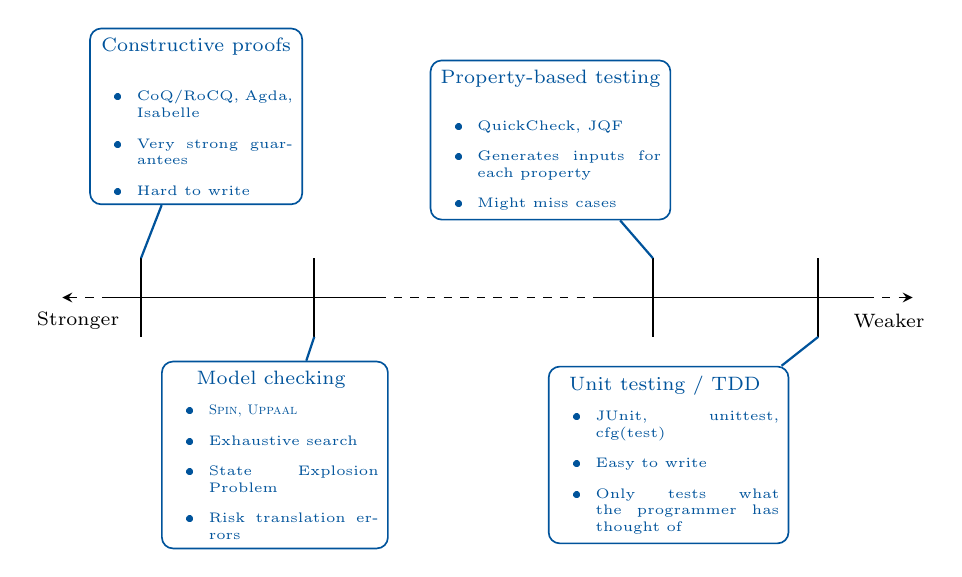
\begin{tikzpicture}[> = stealth, semithick]
    % scale %

    % left half
    \draw [dashed, <-] (-0.2, 0) -- (0.4, 0) ;
    \draw (0.4, 0) -- (3.8, 0) ;

    % middle dashed
    \draw [dashed] (3.8, 0) -- (6.6, 0) ;

    % right half
    \draw (6.6, 0) -- (10, 0) ;
    \draw [dashed, ->] (10, 0) -- (10.6, 0) ;


    % ticks / vertical lines %

    % leftmost tick (constructive proofs)
    \draw<2-> (0.8, -0.5) -- (0.8, 0.5) ;
    
    % tick for model checking
    \draw<3-> (3, -0.5) -- (3, 0.5) ;

    % tick for Quickcheck
    \draw<4-> (7.3, -0.5) -- (7.3, 0.5) ;

    % rightmost tick (unit tests)
    \draw<5-> (9.4, -0.5) -- (9.4, 0.5) ;


    % scale labels %

    \node at (0, -0.3) {\scriptsize Stronger} ;
    \node at (10.3, -0.3) {\scriptsize Weaker} ;


    % text boxes with arrows %

    % constructive proofs
    \node<2->
          [draw, rounded corners,
          text width=7em,
          align=flush center,
          color=staBlue]% 
          at (1.5, 2.3)
          (tbox-prf)
          \bgroup
          \scriptsize
          Constructive proofs
          \vspace*{-2pt}
          \tiny
          % LaTeX looks beautiful and nice
          % Also LaTeX:
          \setlength{\leftmargini}{2em}
          \begin{itemize}%[leftmargin=*]
            \item CoQ/RoCQ, Agda, Isabelle \vspace*{-3pt}
            \item Very strong guarantees \vspace*{-3pt}
            \item Hard to write
          \end{itemize}
          \egroup
          ;
    \draw<2-> [thick, color=staBlue] (tbox-prf) -- (0.8, 0.5) ;

    % model checking
    \node<3->
          [draw, rounded corners,
          text width=7.5em,
          align=flush center,
          color=staBlue]% 
          at (2.5, -2)
          (tbox-mc)
          \bgroup
          \scriptsize
          Model checking
          \vspace*{-3pt}
          \tiny
          \setlength{\leftmargini}{2em}
          \begin{itemize}%[leftmargin=*]
            \item \textsc{Spin, Uppaal}  \vspace*{-3pt}
            \item Exhaustive search  \vspace*{-3pt}
            \item State Explosion Problem  \vspace*{-3pt}
            \item Risk translation errors
          \end{itemize}
          \egroup
          ;
    \draw<3-> [thick, color=staBlue] (tbox-mc) -- (3, -0.5) ;

    % property-based testing
    \node<4->
          [draw, rounded corners,
          text width=8em,
          align=flush center,
          color=staBlue]% 
          at (6, 2)
          (tbox-qc)
          \bgroup
          \scriptsize
          Property-based testing
          \vspace*{-3pt}
          \tiny
          \setlength{\leftmargini}{2em}
          \begin{itemize}%[leftmargin=*]
            \item QuickCheck, JQF \vspace*{-3pt}
            \item Generates inputs for each property \vspace*{-3pt}
            \item Might miss cases
          \end{itemize}
          \egroup
          ;
    \draw<4-> [thick, color=staBlue] (tbox-qc) -- (7.3, 0.5) ;

    % tdd
    \node<5->
          [draw, rounded corners,
          text width=8em,
          align=flush center,
          color=staBlue]% 
          at (7.5, -2)
          (tbox-tdd)
          \bgroup
          \scriptsize
          Unit testing / TDD
          \vspace*{-3pt}
          \tiny
          \setlength{\leftmargini}{2em}
          \begin{itemize}%[leftmargin=*]
            \item JUnit, unittest, cfg(test) \vspace*{-3pt}
            \item Easy to write \vspace*{-3pt}
            \item Only tests what the programmer has thought of
          \end{itemize}
          \egroup
          ;
    \draw<5-> [thick, color=staBlue] (tbox-tdd) -- (9.4, -0.5) ;

  \end{tikzpicture}

\end{frame}


%% MARK: TyDe
\begin{frame}
  \frametitle{What about Type-Driven Development?}

  \begin{itemize}
    \item<1-> Dependently Typed languages like Agda and Idris
    \item<2-> Can construct advanced types and embedded DSLs
    \item<3-> And the type checker then helps verify the program
    \item<4-> Fits somewhere in the middle
  \end{itemize}
\end{frame}


%% MARK: ATM Diagram
\begin{frame}
  \frametitle{The ATM state machine}

  \begin{figure}
    \centering
    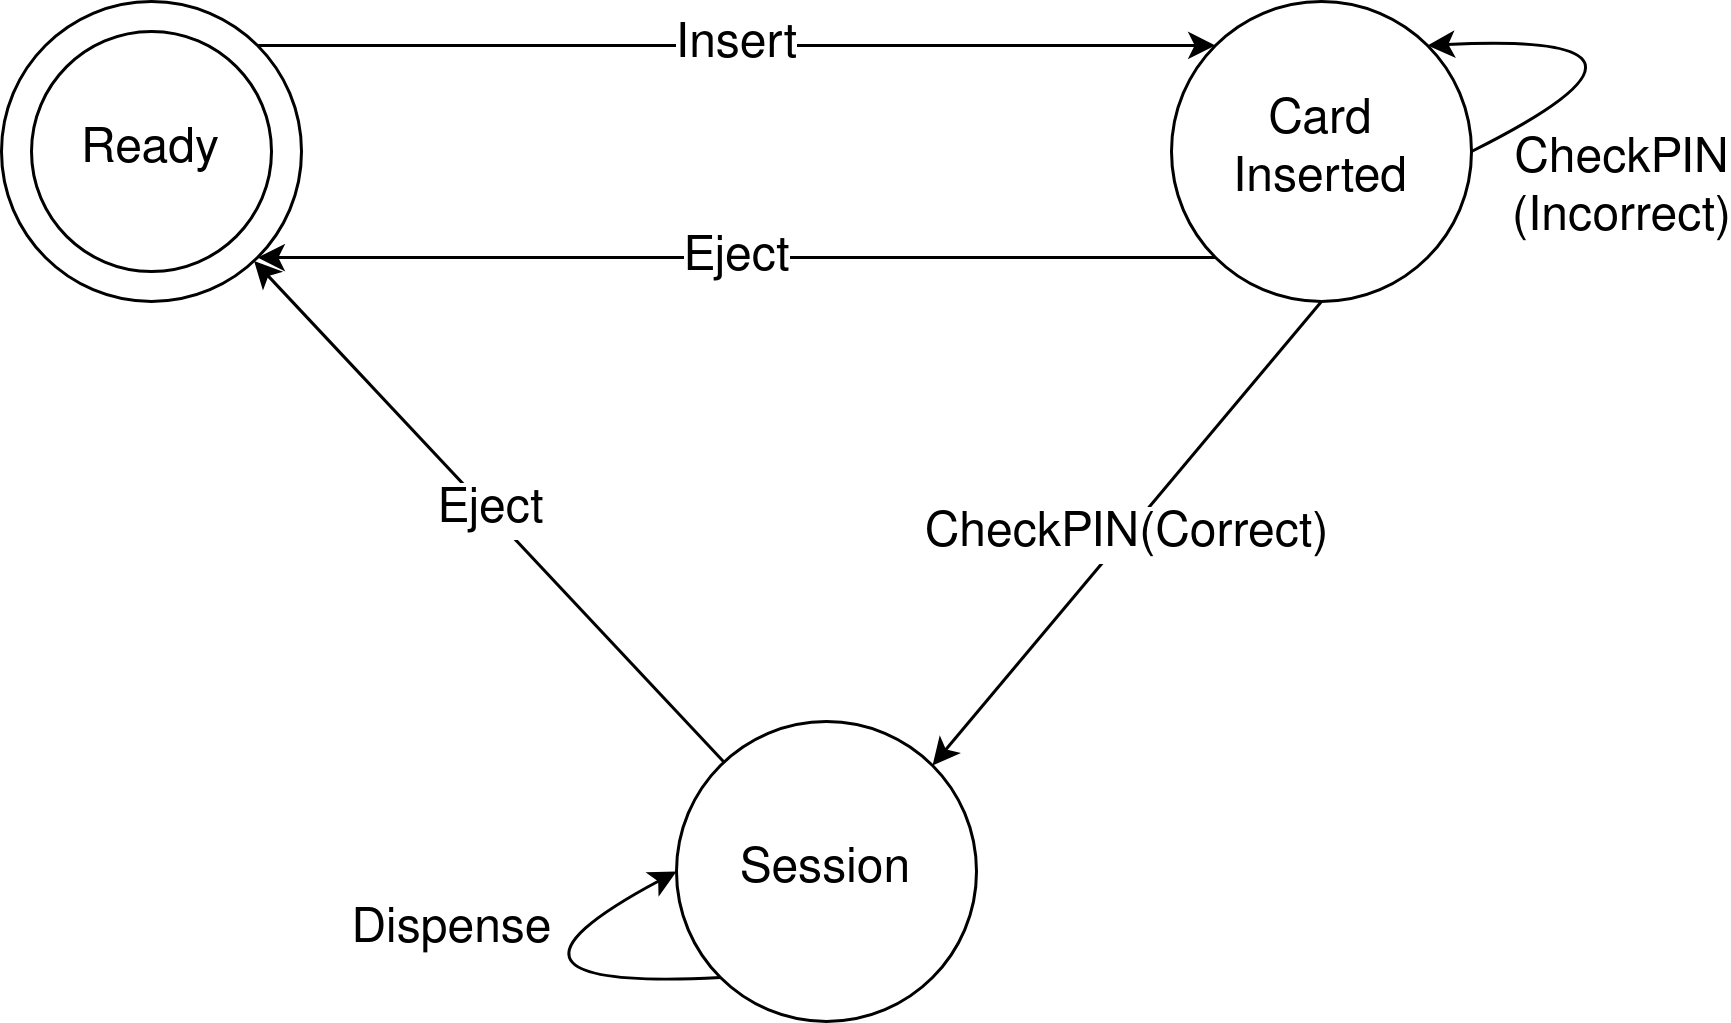
\includegraphics[alt={A state diagram of an ATM, with circles for each state: Ready, CardInserted, and Session; labelled arrows between the states; with the labels containing the transition names: Insert, Dispense, CheckPIN(Correct), CheckPIN(Incorrect), and Eject.},width=0.8\framewidth]{ATM.png}
    %% \Description{A state diagram of an ATM, with circles for each state: Ready,
    %%              CardInserted, and Session; labelled arrows between the states;
    %%              with the labels containing the transition names: Insert,
    %%              Dispense, CheckPIN(Correct), CheckPIN(Incorrect), and Eject.}
  \end{figure}
  \vspace*{-1cm}

\end{frame}


%% MARK: ISM Definition
\begin{frame}
  \frametitle{Model: Indexed State Monads (ISMs)}

  \begin{itemize}
    \item<1-> Declare a datatype for the states
    \item<2-> Declare datatypes for the possible results (if any) of the
              operations
    \item<3-> Declare a datatype with constructors for each operation, such
              that:
      \begin{itemize}
        \item<4-> The type checker can follow the state transitions
        \item<5-> We can program with the operations
      \end{itemize}
  \end{itemize}

\end{frame}


%% MARK: ATM States
\begin{frame}[fragile]
  \frametitle{Datatype for the ATM states}

  \begin{columns}
  \begin{column}{0.3\framewidth}
    \begin{minted}[gobble=6]{Idris}
      data ATMState
        = Ready
        | CardInserted
        | Session
    \end{minted}
  \end{column}

  \begin{column}{0.65\framewidth}
    \begin{figure}
    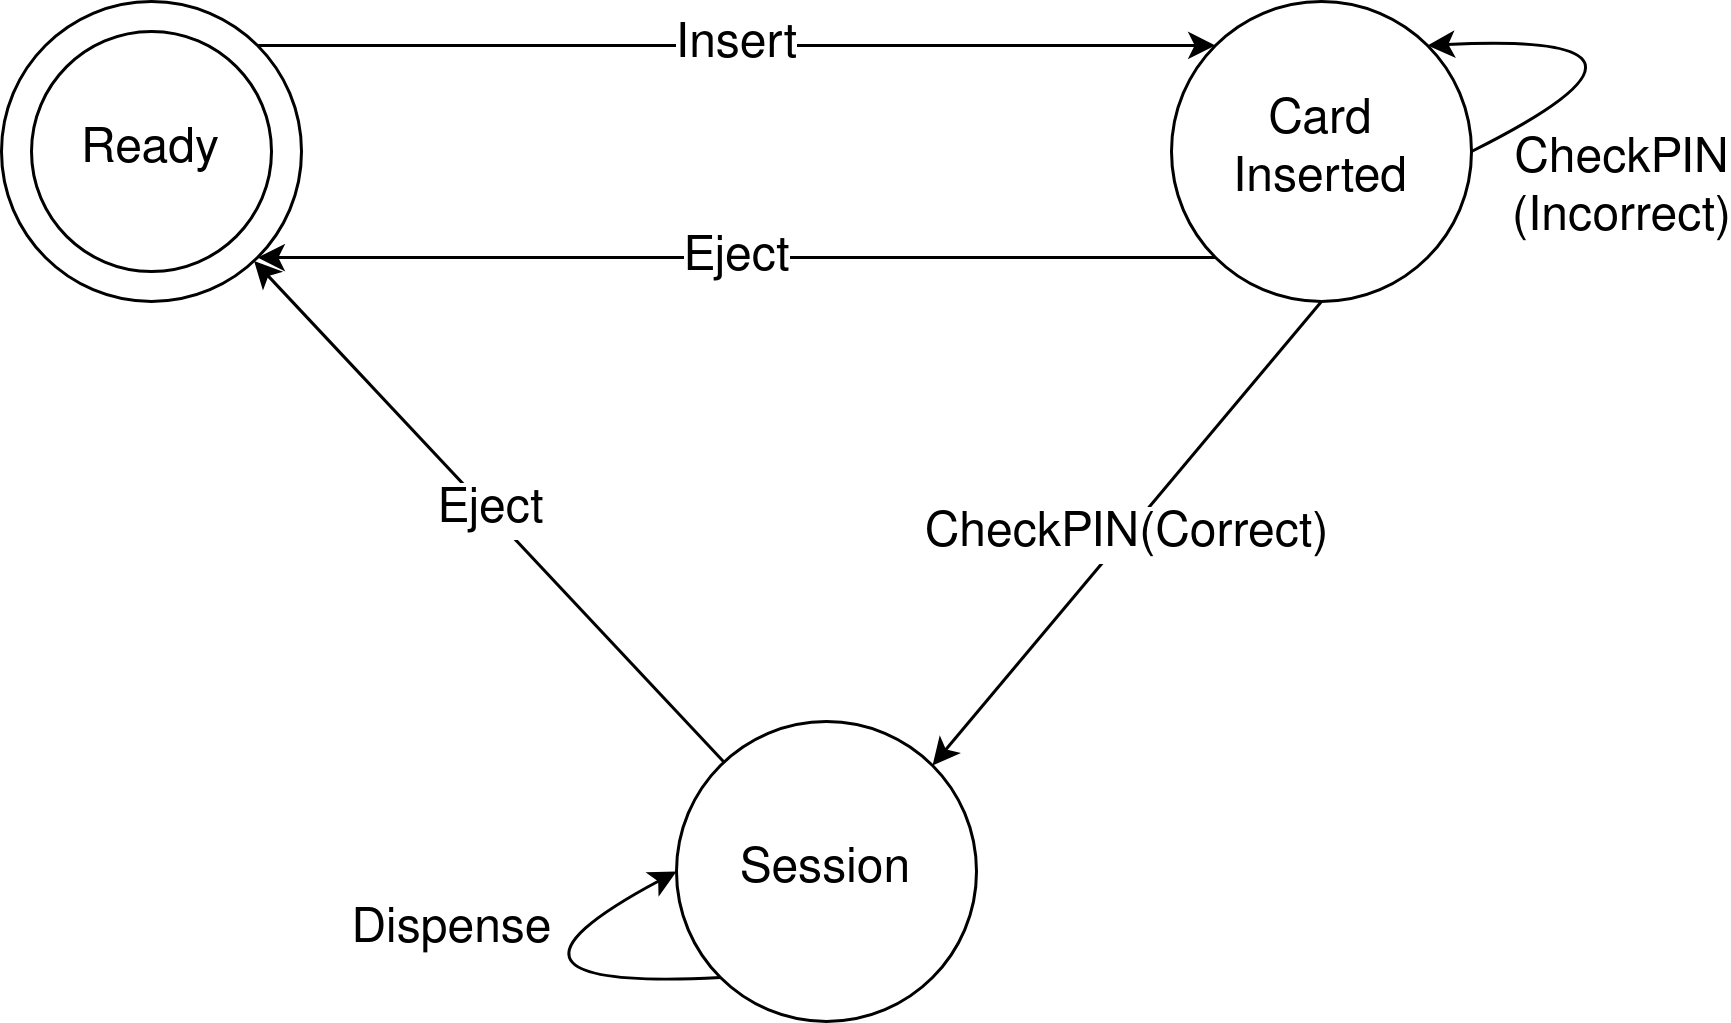
\includegraphics[alt={The state diagram from slide 7.},width=\textwidth]{ATM.png}
    %% \Description{The ATM diagram from slide 7}
    \end{figure}
  \end{column}
  \end{columns}

\end{frame}


%% MARK: ATM Results
\begin{frame}[fragile]
  \frametitle{Datatype for ATM operation results}

  \begin{columns}
  \begin{column}{0.3\framewidth}
    \begin{minted}[gobble=6]{Idris}
      data PINok 
        = Correct
        | Incorrect
    \end{minted}
    \pause
  \end{column}

  \begin{column}{0.65\framewidth}
    \begin{figure}
    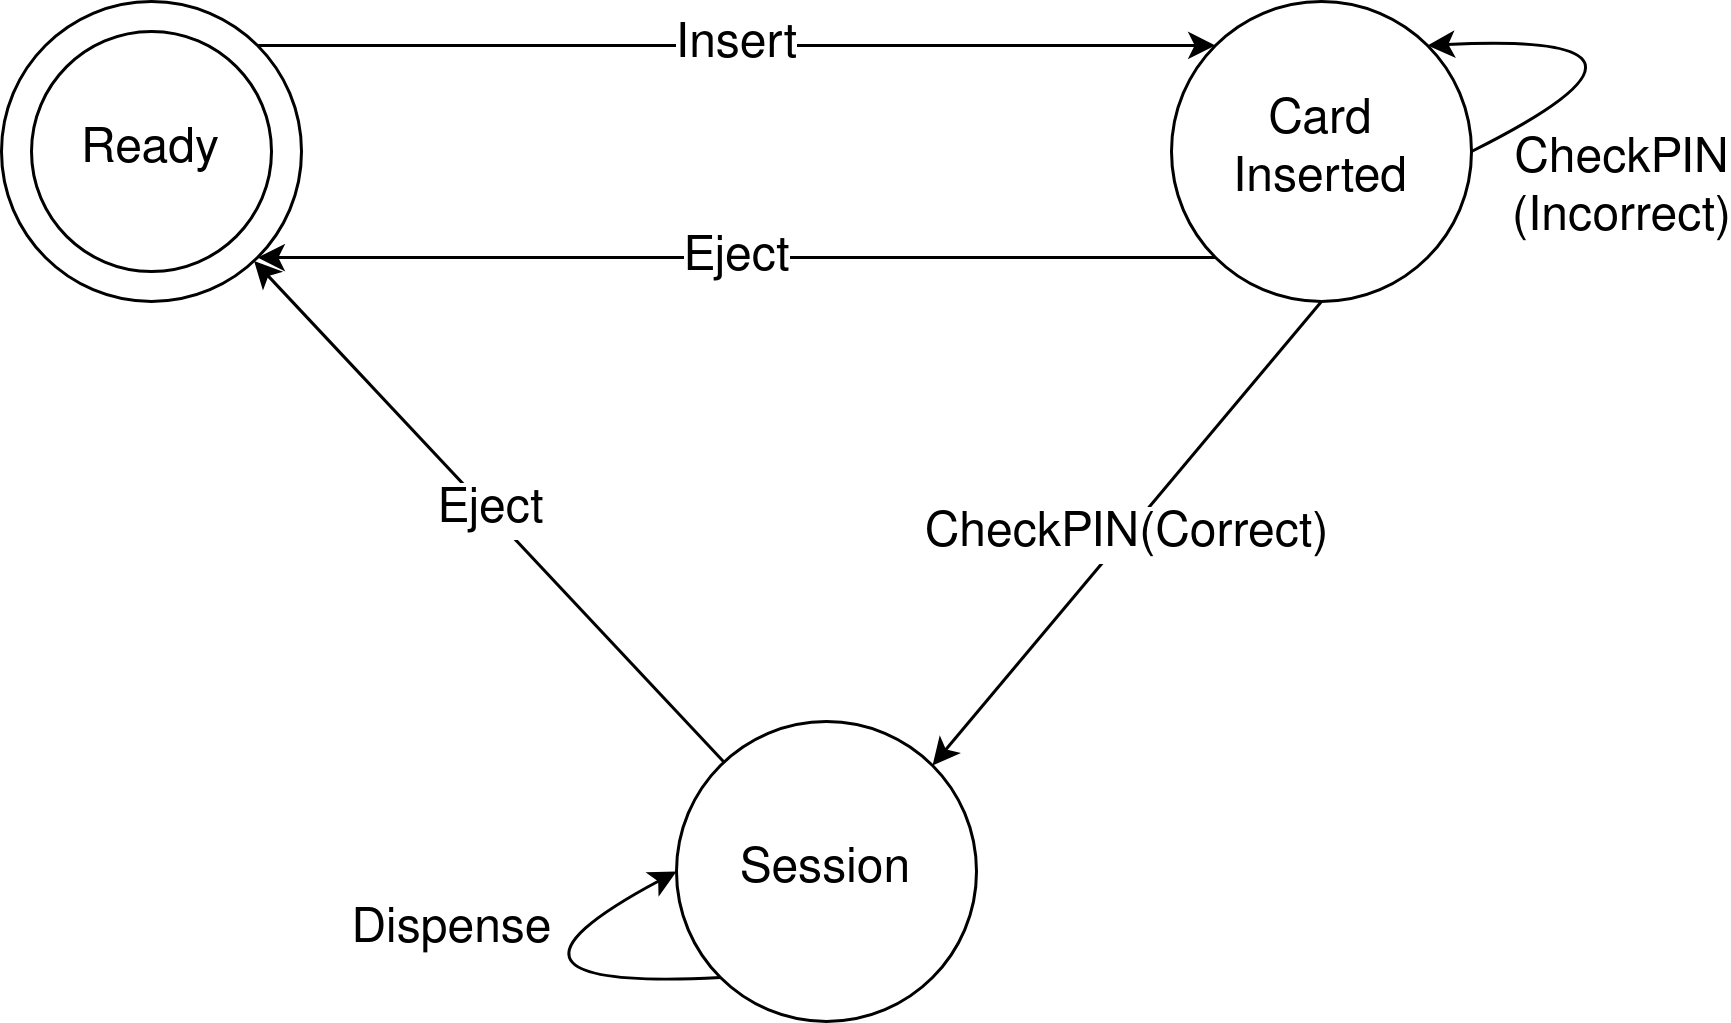
\includegraphics[alt={The state diagram from slide 7.},width=\textwidth]{ATM.png}
    %% \Description{The state diagram from slide 7.}
    \end{figure}
  \end{column}
  \end{columns}

  \vspace*{1cm}

  \pause

  Everything which does not have a result returns Unit {\textemdash}
  \mintinline{Idris}|()|

\end{frame}


\begin{frame}[fragile]
  \frametitle{Dependent State Transition}

  \begin{columns}
  \begin{column}{0.5\framewidth}
    \begin{minted}[gobble=6]{Idris}
      ChkPINfn : PINok -> ATMState
      ChkPINfn Correct = Session
      ChkPINfn Incorrect = CardInserted
    \end{minted}
  \end{column}
  \hspace*{-7mm}
  \begin{column}{0.55\framewidth}
    \begin{figure}
    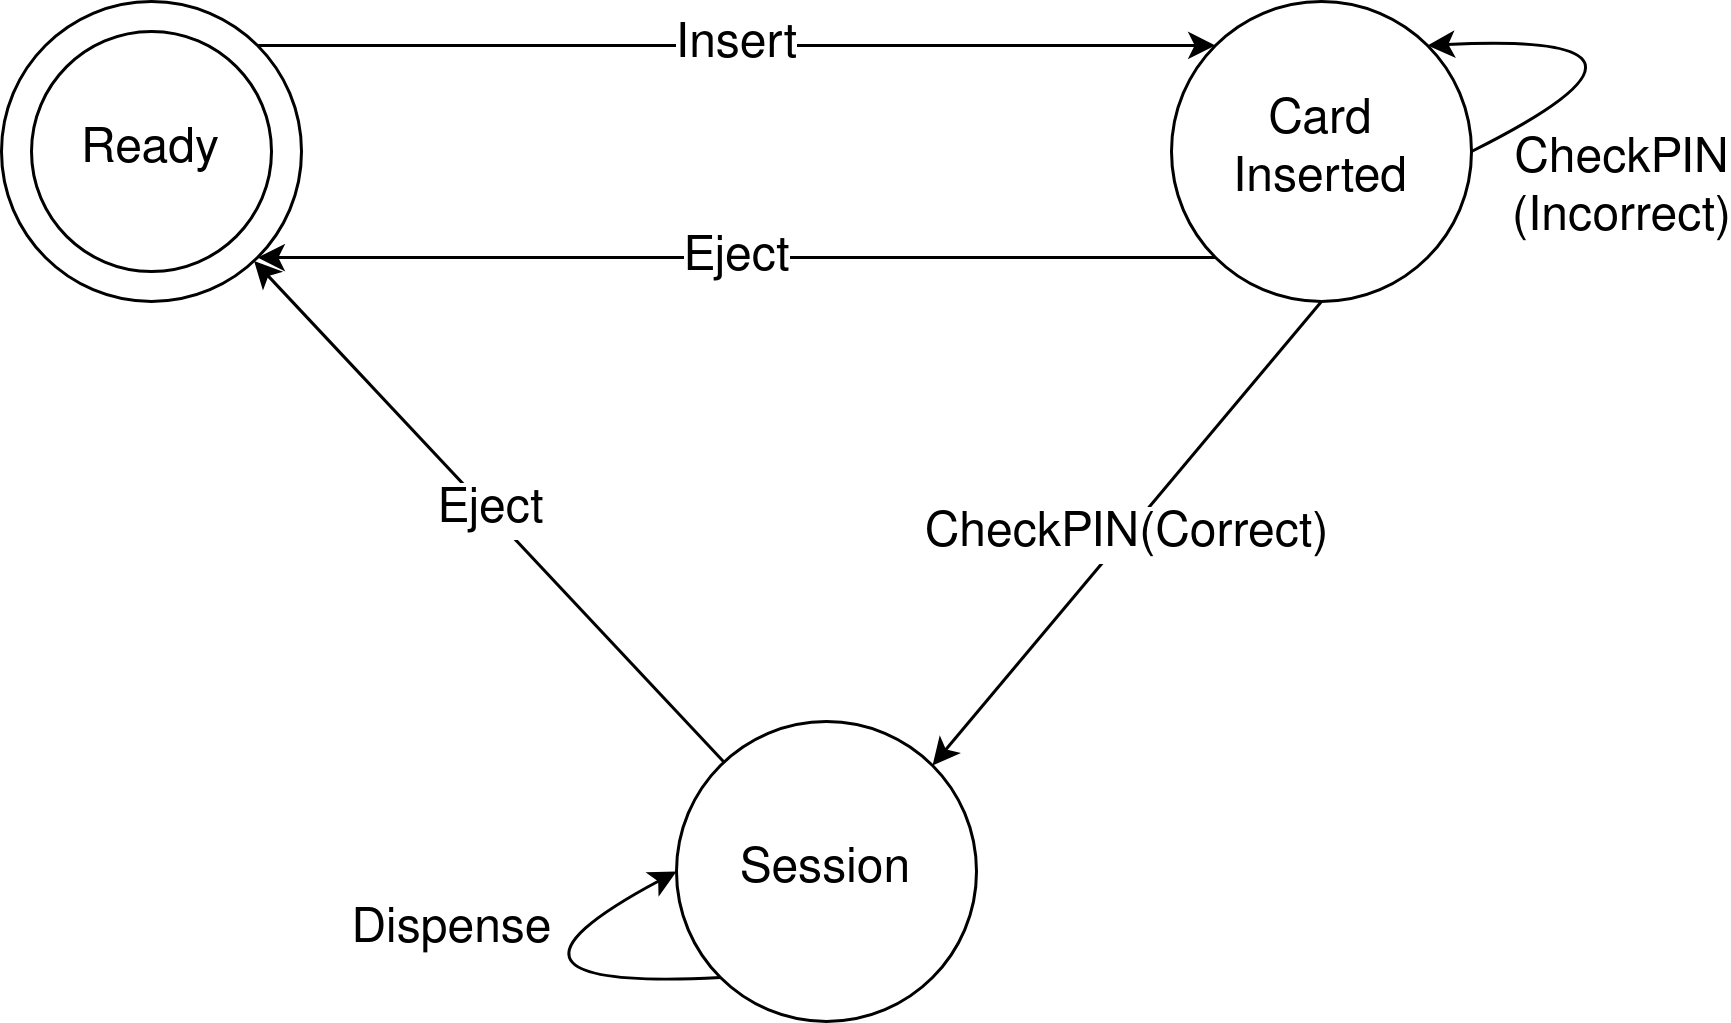
\includegraphics[alt={The state diagram from slide 7.},width=\textwidth]{ATM.png}
    %% \Description{The state diagram from slide 7.}
    \end{figure}
  \end{column}
  \end{columns}

\end{frame}

%% MARK: ATM Operations
\begin{frame}[fragile]
  \frametitle{ATM Indexed State Monad}

  \begin{minted}[gobble=4]{Idris}
    data ATM : (t : Type) -> ATMState -> (t -> ATMState) -> Type where
      Insert : ATM () Ready (const CardInserted)
      CheckPIN : (pin : Int) -> ATM PINok CardInserted ChkPINfn
      Dispense : (amt : Nat) -> ATM () Session (const Session)
      Eject : ATM () st (const Ready)
      Pure : (x : t) -> ATM t (stFn x) stFn
      (>>=) : ATM a s1 s2f -> ((x : a) -> ATM b (s2f x) s3f) -> ATM b s1 s3f
  \end{minted}
\end{frame}


%% MARK: ISM Prog.g
\begin{frame}[fragile]
  \frametitle{Programming with ISMs}

  \begin{itemize}
    \item<1-> We declare our intended start and end state in the type
              \begin{minted}{Idris}
prog : ATM () Ready (const Ready)
              \end{minted}
    \item<2-> And the type-checker verifies that we don't use commands
              incorrectly
              \begin{minted}[breaklines=false]{Idris}
prog = do                    -- We start in Ready
  Insert  --------------------- Ready to CardInserted
  Correct <- CheckPIN 1234  --- CI to Session
    | Incorrect => <...>  ----- (or stay in CI)
  Dispense 42  ---------------- Stay in Session
  Eject  ---------------------- Return to Ready
              \end{minted}
  \end{itemize}

\end{frame}


%% TODO: this is slow and impractical for every stateful program, instead, we
%% can generalise this construct for any ISM


%% MARK: Loop program
\begin{frame}[fragile]
  \frametitle{Dependent Types Only Get Some Things Right}

  \begin{columns}
  \begin{column}{0.47\framewidth}
    {\color{red} Rejected by the type-checker:}
    \vspace*{1mm}
    \begin{minted}[fontsize=\footnotesize]{Idris}
badProg : ATM ()
            Ready (const Ready)
badProg = do
  Insert
  let pin = 1234
  Correct <- CheckPIN pin
    | Incorrect => InsertCard
  Dispense 42
  -- We never Eject, so we
  -- never come back to
  -- `Ready'
    \end{minted}
    \vspace*{2.5mm}
  \end{column}

  \pause  % first show the bad, then the dubious

  \vrule{}

  \begin{column}{0.53\framewidth}
    {\color{orange} Accepted by the type-checker:}
    \vspace*{1mm}
    \begin{minted}[breaklines=false,fontsize=\footnotesize]{Idris}
loopProg : ATM ()
             Ready (const Ready)
loopProg = do
    InsertCard
    let pin = 4321
    loopIncorrect pin
  where
    loopIncorrect : Nat -> ATM ()
                      CardInserted
                      (const Ready)
    loopIncorrect p = do
      Incorrect <- CheckPIN p
        | Correct => -- <...>
      loopIncorrect p
    \end{minted}
    \vspace*{-6mm}
  \end{column}
  \end{columns}
\end{frame}


%% MARK: Why problem?
\begin{frame}
  \frametitle{Why is this a problem?}

  \begin{itemize}
    \item<1-> As-is, the PIN can be brute forced!
    \item<2-> We expect an ATM to reject the card after 3 PIN attempts
    \begin{itemize}
      \item<2-> Not to be permanently unavailable if we retry forever
    \end{itemize}
    \item<3-> However, the programmer is unlikely to catch this
    \item<4-> The model looks correct and rigorous, after all
    \item<5-> Programming with it will catch most errors
    \item<6-> And the type-checker is happy with our sequence of operations
  \end{itemize}
\end{frame}


%% \begin{frame}
%%   \frametitle{How do we solve this?}
%% 
%%   \begin{itemize}
%%     \item<1-> We could spot the issue when it happens
%%     \begin{itemize}
%%       \item<2-> Someone will (hopefully) spot the issue during development
%%       \item<3-> Or, worst case, spot it when it happens after deployment
%%     \end{itemize}
%%     \item<4-> And then we update our model and everything is good
%%     \item<5-> Why not try to spot it \textit{automatically} before either of
%%               those?
%%     \item<6-> Modelling can clearly go wrong, so how do we increase our
%%               confidence in the models?
%%   \end{itemize}
%% \end{frame}


%% \begin{frame}
%%   \frametitle{The eternal problem with verification systems}
%% 
%%   \begin{itemize}
%%     \item<1-> All verification systems face the same problem: ergonomics
%%     \item<2-> If the system is obstructive, or even just perceived as such,
%%               people are unlikely to use it
%%     \item<3-> This is especially true for complex systems
%%     \begin{itemize}
%%       \item<4-> ``Fighting with the Rust borrow-checker''
%%       \item<5-> ``I'm experienced enough to write safe C/C++''
%%       \item<6-> ``I'm experienced enough to get the types right''
%%     \end{itemize}
%%   \end{itemize}
%% 
%% \end{frame}


%% MARK: PBT recap
\begin{frame}
  \frametitle{Suggestion: Property Based Testing}

  \begin{itemize}
    \item<1-> QuickCheck is a Property Based Testing (PBT) framework initially
              developed for Haskell
    \item<2-> Define how to \emph{generate} an instance of a type, given some
              pseudorandom number generator state
      \begin{itemize}
        \item<2-> This is referred to as \mintinline{Idris}{Arbitrary}
      \end{itemize}
    \item<3-> Write \emph{properties} and \emph{generate} their test case inputs
  \end{itemize}

\end{frame}


%% MARK: Gen Vect prob
\begin{frame}[fragile]
  \frametitle{Generating Dependent Types is Tricky}

  \begin{itemize}
    \item<1-> Consider generating arbitrary vectors:
              \begin{minted}[gobble=16]{Idris}
                Arbitrary t => Arbitrary (Vect n t)
              \end{minted}
    \item<2-> \mintinline{Idris}|n| is bound outwith the interface
    \item<3-> We cannot guarantee that the generated \mintinline{Idris}|Vect|
              will have some general, unspecified length \mintinline{Idris}|n|
    \item<4-> We could generate vectors of a specific length, but this is not
              ideal
  \end{itemize}

\end{frame}


\begin{frame}[fragile]
  \frametitle{Arbitrary Dependent Types}

  \begin{itemize}
    \item<1-> The solution is more dependent types!
    \item<2-> Specifically: dependent pairs

    %\vspace*{-1mm}  % <2->
    \begin{minted}{Idris}
record DPair a (p : a -> Type) where
  constructor MkDPair
  fst : a
  snd : p fst
    \end{minted}
    %\vspace*{-1mm}

    \item<3-> As long as we know how to generate an {\textasciigrave
              \mintinline{Idris}{Arbitrary a}\textasciigrave}, we can generate
              an {\textasciigrave
              \mintinline{Idris}{Arbitrary (x : a ** p x)}\textasciigrave}
    \begin{itemize}
      \item<3-> (The \mintinline{Idris}{**} syntax is sugar for
                \mintinline{Idris}{DPair} / \mintinline{Idris}{MkDPair}
                depending on the context)
    \end{itemize}
  \end{itemize}

\end{frame}


\begin{frame}[fragile]
  \frametitle{Arbitrary vectors}

  \begin{itemize}
  \item<1-> Provided we know how to generate the elements, we generate
            \textit{some} length
            \begin{minted}{Idris}
Arbitrary a => Arbitrary (n : Nat ** Vect n a) where
  arbitrary = do
    len <- arbitrary
            \end{minted}
  \item<2-> And then generate that many \mintinline{Idris}{arbitrary}
            elements
            \begin{minted}{Idris}
    vect <- nArbitrary len
    pure (len ** vect)
  where
    nArbitrary : (n : Nat) -> Gen (Vect n a)
    nArbitrary 0 = []
    nArbitrary (S k) = !arbitrary :: nArbitrary k
            \end{minted}
  \vspace*{-5mm}
  \end{itemize}

\end{frame}


\begin{frame}
  \frametitle{Arbitrary ATMs?}

  \begin{itemize}
    \item<1-> Can we do a similar thing for \mintinline{Idris}{ATMOp} and
              \mintinline{Idris}{ATM}?
    \item<2-> Yes, but we need some (dependent) plumbing first
  \end{itemize}

\end{frame}


\begin{frame}[fragile]
  \frametitle{Plumbing for operations}

  \inputminted{Idris}{qc-things/ATM-opres.idr}

\end{frame}


\begin{frame}[fragile]
  \frametitle{Tracing ATMs}

  \inputminted[fontsize=\footnotesize]{Idris}{qc-things/ATM-tracing.idr}

\end{frame}


%%\begin{frame}[fragile]
%%  \frametitle{Generating arbitrary OpRes}
%%
%%  %\vspace*{-2mm}
%%  \inputminted[fontsize=\scriptsize]{Idris}{qc-things/ATM-arb-opres.idr}
%%
%%\end{frame}


\begin{frame}[fragile]
  \frametitle{Arbitrary OpRes: Prerequisites}

  Provided we know what state we are currently in, we can generate an operation
  and its result:

  \begin{minted}{Idris}
{currSt : ATMState} ->
Arbitrary (resT : _ ** nsFn : resT -> ATMState **
           OpRes resT currSt nsFn)
where
          \end{minted}

\end{frame}


\begin{frame}[fragile]
  \frametitle{Arbitrary OpRes: from Ready}

  From \mintinline{Idris}{Ready}, we can insert the card:

  \begin{minted}{Idris}
  arbitrary {currSt=Ready} =
    pure (_ ** _ ** MkOpRes Insert ())
  \end{minted}

\end{frame}


\begin{frame}[fragile]
  \frametitle{Arbitrary OpRes: from CardInserted}

  Using a dummy value for the PIN, we can control the frequencies of the getting
  the PIN right:

  \begin{minted}[fontsize=\footnotesize]{Idris}
arbitrary {currSt=CardInserted} = do
  -- we need a PIN, even though we control the result
  let arbPIN = 0
  let op1 = (_ ** _ ** MkOpRes (CheckPIN arbPIN) Correct)
  let op2 = (_ ** _ ** MkOpRes (CheckPIN arbPIN) Incorrect)
  let op3 = (_ ** _ ** MkOpRes Eject ())

  frequency $ [(1, pure op1), (4, pure op2), (1, pure op3)]
  \end{minted}

\end{frame}


\begin{frame}[fragile]
  \frametitle{Arbitrary OpRes: from Session}

  Generate an arbitrary amount to dispense, or eject the card:

  \begin{minted}{Idris}
arbitrary {currSt=Session} = do
  arbAmount <- arbitrary
  let op1 = (_ ** _ ** MkOpRes (Dispense arbAmount) ())
  let op2 = (_ ** _ ** MkOpRes Eject ())
  oneof [pure op1, pure op2]
  \end{minted}

\end{frame}


\begin{frame}
  \frametitle{Properties of the ATM}

  \begin{itemize}
    \item<1-> Now that we have that, we can specify properties like\\
              ``Within 5 state-transitions, we should be back in
              \mintinline{Idris}{Ready}''
              \vspace*{-1mm}
              \inputminted{Idris}{qc-things/ATM-props.idr}
    \item<2-> \textit{And} we can test it at compile-time
              \vspace*{-1mm}
              \inputminted{Idris}{qc-things/ATM-qc-props.idr}
              \vspace*{-3mm}
  \end{itemize}

\end{frame}


\begin{frame}[fragile]
  \frametitle{Model, verification, and implementation}
  \begin{itemize}
    \item<1-> With most verification tools, we have to translate between models
    \begin{itemize}
      \item<1-> Spec, model, and implementation are independent
    \end{itemize}
    \item<2-> This facilitates translation mistakes
    \begin{itemize}
      \item<2-> Might think we're verifying the same thing, when in actual fact
                the semantics have changed between representations
    \end{itemize}
  \end{itemize}

\end{frame}


\begin{frame}[fragile]
  \frametitle{All in one}

  
  In our case, the specification \textit{is} the model; \textit{everywhere}

  \inputminted[fontsize=\footnotesize]{Idris}{qc-things/ATM-arb-trace.idr}

\end{frame}


\begin{frame}
  \frametitle{QuickCheck spots the error!}

  \begin{itemize}
    \item<1-> If we try to type-check the file we get:
              \vspace*{1mm}
              \inputminted[fontsize=\scriptsize]{Idris}{qc-things/ATM-qc-error.idr}
    \item<2-> And if we investigate by running QC at the REPL, the error is
              exactly the fault in the model:
              \vspace*{1mm}
              \inputminted[fontsize=\scriptsize]{Idris}{qc-things/qc-trace-4.idr}
              \vspace*{-4mm}
  \end{itemize}

\end{frame}


%% TODO: Frame on dep ty.s being ty-lvl prog.s


\begin{frame}[fragile]
  \frametitle{Fixing things}

  \begin{itemize}
    \item<1-> Now that we know there's an error, we can fix things!
              \inputminted[fontsize=\scriptsize]{Idris}{qc-things/ATM-fixed-chkpin.idr}

    \item<2-> Carrying this through to the generators, our QC passes: file reloads
              successfully, the REPL reports
              \begin{minted}[fontsize=\scriptsize]{Idris}
> QuickCheck PROP_eventuallyReady
MkQCRes (Just True) <log> "OK, passed 100 tests"
              \end{minted}
  \end{itemize}

  \vspace*{-3mm}

\end{frame}


%% MARK: Benefits
\begin{frame}
  \frametitle{Benefits of a multifaceted approach}

  \begin{enumerate}
    \item<1-> Adaptability {\textemdash} being able to use different tools
    \item<2-> Speed {\textemdash} can trade speed for level of verification
    \begin{itemize}
      \item<2-> This isn't about proving things, it is about increasing
                confidence in our typed models
    \end{itemize}
    \item<3-> \textbf{Coherence} {\textemdash} all done in one system
      \begin{itemize}
        \item<4-> No need to translate to model-checking tool
        \item<5-> Specification lives alongside model lives alongside
                  implementation
        \item<6-> The implementation is just there; it \emph{is} runnable code
        \item<7-> Parts can be verified independently \emph{while} combined into an
                  overall system
      \end{itemize}
  \end{enumerate}

\end{frame}


%% FIXME: is this necessary?
%%
%% \begin{frame}
%%   \frametitle{Conclusion}
%% 
%%   \begin{itemize}
%%     \item<1-> Many verification tools exist, none of them cover enough on their
%%               own
%%     \item<2-> Instead of ``competing'', we combine the systems to work together
%%     \item<3-> Hopefully this will lead to wider adoption and better whole-system
%%               soundness
%%   \end{itemize}
%% 
%% \end{frame}


\begin{frame}
  \frametitle{Further work}

  \begin{itemize}
    \item<1-> Running tests at the type level puts a lot of strain on the
              compiler, so there may be interesting optimisations to explore
              there
    \item<2-> Can we do more? ARQ with Sliding Window? Protocols with crash-stop
              failures?
    \item<3-> What kinds of properties can we test? Model Checking has been
              mentioned several times, so how does this compare to LTL or
              TLA\textsuperscript{+}?
  \end{itemize}

\end{frame}


\begin{frame}

  \begin{center}
    \textcolor<1>{staDarkGreen}{\Large Thank you}
  \end{center}

\end{frame}


\begin{frame}
  \frametitle{Links}

  \todo{PAPER, CODE, SLIDES}

  \begin{center}
    Contact: {\href{mailto:teh6@st-andrews.ac.uk}{teh6@st-andrews.ac.uk}}
  \end{center}

  \begin{columns}
  \begin{column}{0.3\framewidth}
    \begin{center}
      Preprint
      \begin{figure}
        
\includegraphics[width=\textwidth]{arxiv-qr.png}
      \end{figure}
      \href{https://doi.org/10.48550/arXiv.2407.12726}{arXiv:2407.12726}
    \end{center}
  \end{column}
  \begin{column}{0.3\framewidth}
    \begin{center}
      Code
      \begin{figure}
        
\includegraphics[width=\textwidth]{code-qr.png}
      \end{figure}
      \href{https://github.com/CodingCellist/tyde-24-code}{GH: CodingCellist/tyde-24-code}
    \end{center}
  \end{column}
  \begin{column}{0.3\framewidth}
    \begin{center}
      Slides
      \begin{figure}
        %% \includegraphics[width=\textwidth]{imagefile}
      \end{figure}
    \end{center}
  \end{column}
  \end{columns}

  %% \begin{center}
  %%   \begin{figure}
  %%     
\includegraphics[width=0.30\framewidth]{qr-code.png}
  %%     \caption{\href{https://github.com/CodingCellist/talks/tree/main/2024-03-06-spls-st-andrews}{github.com/CodingCellist/talks}}
  %%   \end{figure}
  %%   {\href{mailto:teh6@st-andrews.ac.uk}{\small teh6@st-andrews.ac.uk}}
  %%   \vspace*{-10mm}
  %% \end{center}

\end{frame}

\end{document}

